\documentclass{beamer}
\usepackage{tikz,amsmath,hyperref,graphicx,stackrel,animate,media9}
\usetikzlibrary{positioning,shadows,arrows,shapes,calc}
\newcommand{\argmax}{\operatornamewithlimits{argmax}}
\newcommand{\argmin}{\operatornamewithlimits{argmin}}
\mode<presentation>{\usetheme{Frankfurt}}
\AtBeginSection[]
{
  \begin{frame}<beamer>
    \frametitle{Outline}
    \tableofcontents[currentsection,currentsubsection]
  \end{frame}
}
\title{Lecture 6: Operations on Periodic Signals}
\author{Mark Hasegawa-Johnson}
\date{ECE 401: Signal and Image Analysis}
\begin{document}

% Title
\begin{frame}
  \maketitle
\end{frame}

% Title
\begin{frame}
  \tableofcontents
\end{frame}

%%%%%%%%%%%%%%%%%%%%%%%%%%%%%%%%%%%%%%%%%%%%
\section[Spectrum]{Review: Spectrum}
\setcounter{subsection}{1}

\begin{frame}
  \frametitle{Two-sided spectrum}

  The {\bf spectrum} of $x(t)$ is the set of frequencies, and their
  associated phasors,
  \[
  \mbox{Spectrum}\left( x(t) \right) =
  \left\{ (f_{-N},a_{-N}), \ldots, (f_0,a_0), \ldots, (f_N,a_N) \right\}
  \]
  such that
  \[
  x(t) = \sum_{k=-N}^N a_ke^{j2\pi f_kt}
  \]
\end{frame}

\begin{frame}
  \frametitle{Properties of the Spectrum}
  \begin{itemize}
  \item {\bf Scaling:}
    \[
    y(t) = Gx(t)\Leftrightarrow a_k \rightarrow Ga_k
    \]
  \item {\bf Add a Constant:}
    \[
    y(t)=x(t)+C \Leftrightarrow
    a_k \rightarrow \begin{cases}
      a_0+C & k=0 \\
      a_k & \mbox{otherwise}
    \end{cases}
    \]
  \item {\bf Add Signals:} Suppose that the $n^{\textrm{th}}$ frequency
    of $x(t)$, $m^{\textrm{th}}$ frequency of $y(t)$, and
    $k^{\textrm{th}}$ frequency of $z(t)$ are all the same frequency.  Then 
    \[
    z(t)=x(t)+y(t)
    \Leftrightarrow
    a_k \rightarrow a_n+a_m
    \]
  \end{itemize}
\end{frame}

\begin{frame}
  \frametitle{Properties of the Spectrum}
  \begin{itemize}
  \item {\bf Time Shift:} Shifting to the right, in time, by $\tau$
    seconds:
    \[
    y(t)=x(t-\tau)\Leftrightarrow a_k\rightarrow a_k e^{-j2\pi f_k\tau}
    \]
  \item {\bf Frequency Shift:} Shifting upward in frequency by $F$
    Hertz:
    \[
    y(t)=x(t)e^{j2\pi Ft} \Leftrightarrow f_k\rightarrow f_k+F
    \]
  \item {\bf Differentiation:}
    \[
    y(t) = \frac{dx}{dt} \Leftrightarrow a_k\rightarrow j2\pi f_k a_k
    \]
  \end{itemize}
\end{frame}  

%%%%%%%%%%%%%%%%%%%%%%%%%%%%%%%%%%%%%%%%%%%%
\section[Fourier Series]{Spectral Properties of a Fourier Series}
\setcounter{subsection}{1}

\begin{frame}
  \frametitle{Fourier Analysis and Synthesis}
  \begin{itemize}
  \item {\bf Fourier Analysis}  (finding the spectrum, given the waveform):
    \[
    X_k = \frac{1}{T_0}\int_0^{T_0} x(t)e^{-j2\pi kt/T_0}dt
    \]
  \item {\bf Fourier Synthesis}  (finding the waveform, given the spectrum):
    \[
    x(t) = \sum_{k=-\infty}^\infty X_k e^{j2\pi kt/T_0}
    \]
  \end{itemize}
\end{frame}  

\begin{frame}
  \frametitle{Fourier Analysis and Synthesis}
  Compare this:
  \[
  x(t) = \sum_{k=-\infty}^\infty X_k e^{j2\pi kt/T_0}
  \]
  to this:
  \[
  x(t) = \sum_{k=-N}^N a_ke^{j2\pi f_kt}
  \]
  we see that a Fourier series is a spectrum in which the
  $k^{\textrm{th}}$ frequency is $f_k=kF_0$, and the $k^{\textrm{th}}$
  phasor is $a_k=X_k$.
\end{frame}  

\begin{frame}
  \frametitle{Scaling Property for Fourier Series}
  The scaling property for spectra is
  \[
  y(t) = Gx(t)\Leftrightarrow a_k \rightarrow Ga_k
  \]
  Plugging in $f_k=kF_0$ and $a_k=X_k$, we get
  \[
  y(t) = Gx(t) \Leftrightarrow Y_k = GX_k
  \]
\end{frame}

\begin{frame}
  \frametitle{Constant Offset Property}
  \[
  y(t)
  =x(t)+C
  \Leftrightarrow
  a_k \rightarrow
  \begin{cases}
    a_0+C&k=0\\
    a_k&\mbox{otherwise}
  \end{cases}
  \]
  Plugging in $f_k=kF_0$ and $a_k=X_k$, we get
  \[
  y(t)=x(t)+C\Leftrightarrow
  Y_k =
  \begin{cases}
    X_0+C&k=0\\
    X_k&\mbox{otherwise}
  \end{cases}
  \]
\end{frame}
\begin{frame}
  \frametitle{Signal Addition Property}

  Suppose that $x(t)$ and $y(t)$ have the same fundamental frequency, $F_0$.
  In that case they have the same frequencies $f_k=kF_0$ in their spectra, so
  \[
  z(t)=x(t)+y(t) \Leftrightarrow Z_k = X_k+Y_k
  \]
\end{frame}

\begin{frame}
  \frametitle{Time Shift Property for Fourier Series}

  The {\bf Time Shift} property of a spectrum is that, if you shift
  the signal $x(t)$ to the right by $\tau$ seconds, then:
  \[
  y(t)=x(t-\tau)\Leftrightarrow a_k\rightarrow a_k e^{-j2\pi f_k\tau}
  \]
  Plugging in $f_k=kF_0$ and $a_k=X_k$, we get
  \[
  y(t)=x(t-\tau)\Leftrightarrow Y_k= X_k e^{-j2\pi kF_0\tau}
  \]
\end{frame}

\begin{frame}
  \frametitle{Frequency Shift Property for Fourier Series}

  The {\bf Frequency Shift} property for spectra says that if we
  multiply by a complex exponential in the time domain, that shifts
  the entire spectrum by $F$:
  \[
  y(t)=x(t)e^{j2\pi Ft} \Leftrightarrow f_k\rightarrow f_k+F
  \]
  Suppose that the shift frequency is $F=dF_0$, i.e., it's
  some integer, $d$, times the fundamental.
  Then
  \begin{itemize}
  \item The phasor $X_k$ is no longer active at $kF_0$;
    instead, now it's active at $(k+d)F_0$
  \item We can say that $Y_k$, the phasor at frequency $kF_0$, is
    the same as $X_{k-d}$, the phase at frequency $(k-d)F_0$.
  \end{itemize}
  \[
  y(t)=x(t)e^{j2\pi Ft} \Leftrightarrow Y_{k} = X_{k-d}
  \]
\end{frame}
\begin{frame}
  \frametitle{Differentiation Property for Fourier Series}
  The {\bf Differentiation} property for spectra is
  \[
  y(t) = \frac{dx}{dt} \Leftrightarrow a_k\rightarrow j2\pi f_k a_k
  \]
  If we plug in $f_k=kF_0$ and $a_k=X_k$, we get
  \[
  y(t) = \frac{dx}{dt} \Leftrightarrow Y_k= j2\pi kF_0 X_k
  \]
  So differentiation in the time domain means multiplying by $k$ in
  the frequency domain.
\end{frame}  

\begin{frame}
  \frametitle{Quiz}

  Try the quiz! Go to the course webpage, and click on today's date.
\end{frame}

%%%%%%%%%%%%%%%%%%%%%%%%%%%%%%%%%%%%%%%%%%%%
\section[Time-Varying]{Signals with Time-Varying Fundamental Frequencies}
\setcounter{subsection}{1}

\begin{frame}
  \frametitle{Spectrogram}

  Many signals have time-varying fundamental frequencies.  We show
  their spectral content by doing Fourier analysis once per 10ms or
  so, and plotting the log-magnitude Fourier series coefficients as an
  image called a {\bf spectrogram.}  For example, the spectrogram
  below is from part of Nicholas James Bridgewater's reading of the
  \href{http://ia800201.us.archive.org/4/items/human_rights_3_librivox/human_rights_03_eng_njb.mp3}{\color{blue}Universal Declaration of Human Rights}
  
  \centerline{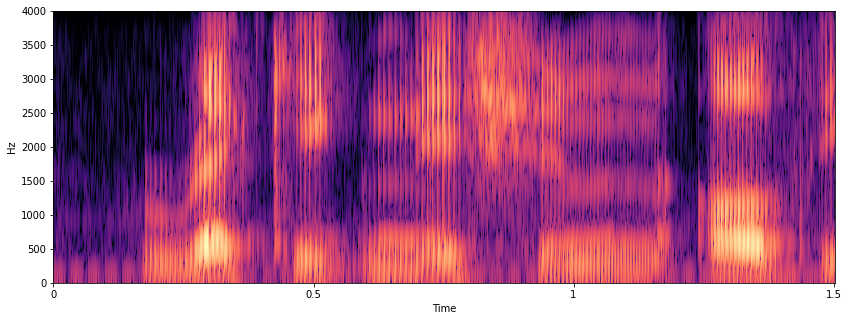
\includegraphics[width=3in]{recognitionofthe.png}}
\end{frame}

\begin{frame}
  \frametitle{Spectrogram}

  The \href{https://dspfirst.gatech.edu/chapters/03spect/demos/spectrog/index.html}{\color{blue}textbook demo page on spectrograms} has more good examples.
\end{frame}

\begin{frame}
  \frametitle{Chirp}

  You might not have noticed this, but we can write a pure tone as
  \[
  x(t) = e^{j\phi}
  \]
  where $\phi = 2\pi f t$ is the instantaneous phase.  Notice that
  the relationship between frequency and phase is
  \[
  f = \frac{1}{2\pi} \frac{d\phi}{dt}
  \]
\end{frame}
\begin{frame}
  \frametitle{Chirp}

  In the same way, we can usefully describe the {\bf instantaneous
    frequency} of a chirp.  For example, consider the linear chirp signal:
  \[
  x(t) = e^{ja t^2}
  \]
  In this case, $\phi=at^2$, so 
  \[
  f = \frac{1}{2\pi} \frac{d\phi}{dt} = \frac{a}{2\pi} t
  \]
  The frequency is now changing as a function of time.  Please look at the
  \href{https://dspfirst.gatech.edu/chapters/03spect/demos/spectrog/chirps/}{\color{blue}textbook demo page}
  for more cool examples.
\end{frame}


%%%%%%%%%%%%%%%%%%%%%%%%%%%%%%%%%%%%%%%%%%%%
\section[Summary]{Summary}
\setcounter{subsection}{1}

\begin{frame}
  \frametitle{Spectral Properties of Fourier Series}
  \begin{itemize}
  \item {\bf Scaling:}
    \[
    y(t) = Gx(t)\Leftrightarrow Y_k = GX_k
    \]
  \item {\bf Add a Constant:}
    \[
    y(t)=x(t)+C \Leftrightarrow
    Y_k = \begin{cases}
      X_0+C & k=0 \\
      X_k & \mbox{otherwise}
    \end{cases}
    \]
  \item {\bf Add Signals:} Suppose that $x(t)$ and $y(t)$ have the
    same fundamental frequency, then
    \[
    z(t)=x(t)+y(t)
    \Leftrightarrow
    Z_k = X_k+Y_k
    \]
  \end{itemize}
\end{frame}  

\begin{frame}
  \frametitle{Spectral Properties of Fourier Series}
  \begin{itemize}
  \item {\bf Time Shift:} Shifting to the right, in time, by $\tau$
    seconds:
    \[
    y(t)=x(t-\tau)\Leftrightarrow Y_k= X_k e^{-j2\pi kF_0\tau}
    \]
  \item {\bf Frequency Shift:} Shifting upward in frequency by $F$
    Hertz:
    \[
    y(t)=x(t)e^{j2\pi dF_0t} \Leftrightarrow Y_k= X_{k-d}
    \]
  \item {\bf Differentiation:}
    \[
    y(t) = \frac{dx}{dt} \Leftrightarrow Y_k= j2\pi kF_0 X_k
    \]
  \end{itemize}
\end{frame}  
        
\end{document}
